%!TEX root = ../dokumentation.tex

\chapter{Theoretische Grundlagen}\label{cha:Grundlagen}
Kurze Einleitung in das Kapitel. Beschreiben warum die Grundlagen notwendig sind. Auch darüber schreiben, dass nicht ALLE Grundlagen sondern lediglich die für das Verständnis der Arbeit notwendigen erklärt werden.

\section{Überwachung von IT-Infrastrukturen}\label{sec:UeberwachungIT}
Worum geht es bei der Überwachung? Was ist das Ziel? Warum braucht man eine Überwachung? Wie sieht diese i.d.R. Aus? Welche Kernpunkte gibt es in der Überwachung? \\
Hier sollte die Überleitung zum nächsten Kapitel kommen d.h. Logfiles werden als letztes behandelt in diesem Kapitel, damit der Übergang sauber ist.

\section{Bedeutung von Logfiles}\label{sec:BedeutungVonLogfiles}
Was sind Logfiles im allgemeinen? Was ist die Funktion eines Logfiles? Gibt es Standards? Wenn ja welche und wie sehen die aus? Werden die Standards im weiteren Verlauf der Arbeit noch einmal relevant sein (Ja/Nein begründen und erläutern)?

\section{Einführung in MapReduce}\label{sec:EinführungInMapReduce}
Die Google Mitarbeiter Jeffrey Dean und Sanjar Ghemawat standen veröffentlichten 2004 eine Arbeit, in welcher sie einen neuen Ansatz zur Verarbeitung von großen, unstrukturierten Daten beschrieben. Das in der Arbeit beschriebene Modell wurde als \textit{Map-Reduce} bezeichnet. Dabei wurde nicht nur beschrieben, wie man große Datenmengen durchsucht, auswetet und in Schlüssel-Wert-Paaren zusammenfast. Die Clusterung von Jobs auf \gls{Commodity-Hardware} waren ebenfalls ein Bestandteil der Arbeit. Freiknecht schreibt weiter, dass diese Arbeit als Ursprung des Algorithmus bezeichnet wird, und somit Implementierungen wie Hadoop, Disco oder BashReduce inspiriert hat.\footcite[Vgl.][S. 42]{Freiknecht.2014}

Ein MapReduce Programm lässt sich i.d.R. in drei Bereiche unterteilen. Der Map-Phase, in welcher die Schlüssel-Wert-Paare aus den Eingabedaten erzeugt werden, der Combine-Phase, zur Aggregation der Paare, sowie der Reduce-Phase, in welcher die Daten ausgedünnt werden, bis nur noch ein Wert pro Schlüssel vorhanden ist (siehe \autoref{fig:DreiPhasenMapReduce}).

\begin{figure}[h]
	\centering
	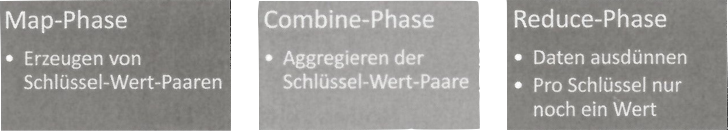
\includegraphics[width=.8\textwidth]{MapReduce_001.png}
	\caption{Die drei Phasen eines Map-Reduce-Prozesses\footnotemark}
	\label{fig:DreiPhasenMapReduce}
\end{figure}
\footnotetext{S. 42 \cite{Freiknecht.2014}}

Woher kommt MapReduce? Wie funktioniert MapReduce? Stärken/Schwächen aufzeigen. Versuchen den Algorithmus mathematisch zu beschreiben ($O(n)$ Methode, Mengenleere). Hierfür muss noch Literatur gesucht werden. Bisher nur mathematische Beschreibungen im Internet gefunden.

\begin{equation}
	V = \frac{1}{2} \tau \cdot r^{2} \cdot h
\end{equation}

\section{Was ist Hadoop?}\label{sec:WasIstHadoop}
\flqq Kurz gesagt: Hadoop ist ein freies, Java-basiertes Open-Source-Framework für die skalierbare und verteilte Verarbeitung großer Datenmengen auf vielen Rechnern innerhalb eines Netzwerks.\frqq\footcite[S. 21]{Wartala.2012}

Die Entwicklung begann im Jahr 2004 durch den Programmierer Doug Cutting, nachdem dieser, im Rahmen des 6. Symposiums \textit{Operating Systems Design and Implementations} (\acs{OSDI}), den Vortrag "`MapReduce - Simplified Data Processing on Large Clusters"', von den Google Mitarbeitern Jeffrey Dean und Sanjay Ghemawat, gehört hatte.

Zu diesem Zeitpunkt arbeitete Cutting an seinem Suchmaschienenprojekt mit dem Namen "`Nutch"', welches bereits 2002 ins leben gerufen wurde. Sein Ziel war eine leistungsfähige und konkurrenzfähige Softwarearchitektur, die es mit kommerziellen Suchmaschienen aufnehmen konnte. Bis 2004 konnte Nutch bereits 100 Mio. Webseiten mit nur vier Rechnerknoten indexieren.

Um jedoch das gesamte World Wide Web indexieren zu können, suchte Cutting gemeinsam mit der Nutch-Community nach einer Möglichkeit, die zugrundeliegende Architektur noch skalierbarer zu machen. Nach dem Vortrag bei der \acs{OSDI} fand Cutting eine passende Systemarchitektur in einem ebenfalls durch Dean und Ghemawat veröffentlichten Ansatz.\footcite[Näheres siehe][]{Dean.2004}

Gemeinsam mit zwei Teilzeit-Programmierern implementierte er ein, durch das Google Dateisystem \ac{GFS} inspiriertes, verteiltes Dateisystem, um darauf den MapReduce-Ansatz unter Nutch zu realisieren. 2006 wechselte Cutting zu Yahoo!. Das Dateisystem und MapReduce-Framework wurde aus Nutch extrahiert und in das eigenständige Apache-Projekt Hadoop überführt. Heute wird Hadoop in einer Reihe von Unternehmen produktiv eingesetzt, darunter Yahoo!, IBM und Microsoft.\footnote{Referenzzahlen für Unternehmen, die Hadoop einsetzen, unter:\\ \url{http://wiki.apache.org/hadoop/PoweredBy}}

Hadoop besteht aus zwei Kernkomponenten. Dem verteilten Dateisystem \ac{HDFS} und dem MapReduce-Framework. Dabei wird keine spezielle Servertechnik benötigt. Hadoop lässt sich sehr leicht auf Standardhardware betreiben.\footcite[Vgl.][S. 19-22]{Wartala.2012}

Die einzlenen Komponenten sind unabhängig voneinander einsetzbar. Eine große Rolle spielt bei Hadoop das Konzept der Datenlokalität. Entgegen dem normalen vorgehen, bei welchem einem Programm die daten zu verfügung gestellt werden, wird bei Hadoop das Programm zur Ausführung im Cluster verteilt. Da es sich bei Hadoop i.d.R. um Anwendungen im Big Data bereich handelt, macht es Sinn, da die Anwendung wesentlich kleiner und somit schneller zu übertragen ist, als die Daten.\footcite[Vgl.][S. 20]{Freiknecht.2014}

\subsection{Das verteilte Dateisystem HDFS}\label{subsec:DasVerteilteDateisystemHDFS}
Was ist ein verteiltes Dateisystem überhaupt und wozu braucht man es? Vergleich mit einem normalen Dateisystem?

\subsection{MapReduce-Framework}\label{subsec:MapReduceFramework}
ACHTUNG. Vermutlich überflüssig da MapReduce bereits beschrieben wurde. Das Framework funktioniert nicht wirklich anders es stellt nur interfaces bereit damit die klassen stimmen.

\subsection{Abgrenzung - Was ist Hadoop nicht?}

%Was gehört alles zu Hadoop? Worauf zieht Hadoop ab? Warum verwende ich Hadoop statt es einfach selbst zu machen? Stärken und Schwächen aufzeigen.

%\section{Betrachten von Alternativen}
%Alternativen sowohl zu Hadoop als auch zu MapReduce selbst. Was gibt es in diesen Bereichen noch? Wie unterscheiden sich diese?
%TODO: Alternativen in 3.3 und 5.1 oder eher 5.4 betrachten/erwähnen